\documentclass{beamer}
\usepackage[utf8]{inputenc}

\usetheme[minimal]{NITK}

% -------------------------------------------------------------------------------------------------------------------------------------------
% 																			TITLE
% -------------------------------------------------------------------------------------------------------------------------------------------
\title[Cool Project Presentation]{\bfseries{A Cool Title for My Project}}
\subtitle{I did not clone from GitHub}

\author[Adke \& Alex]{Adke\inst{1} \and Alex\inst{2}}

\institute[NITK]
{
  \inst{1}
  Department of Electrical and Electronics Engineering\\
  National Institute of Technology Karnataka
  \and
  \inst{2}
  Department of Chemical Engineering\\
  National Institute of Technology Karnataka
}

\date[ICIP, 2019]{International Conference on Awesomeness\\April 1st, 2019}


\AtBeginSection[]
{
  \begin{frame}
    \frametitle{Table of Contents}
    \tableofcontents[currentsection]
  \end{frame}
}

% -------------------------------------------------------------------------------------------------------------------------------------------
% 																			CONTENTS
% -------------------------------------------------------------------------------------------------------------------------------------------
\begin{document}

\frame{\titlepage}

\begin{frame}
\frametitle{Table of Contents}
\tableofcontents
\end{frame}

% -------------------------------------------------------------------------------------------------------------------------------------------
% 																			INTRO
% -------------------------------------------------------------------------------------------------------------------------------------------
\section{Introduction}

\begin{frame}
\frametitle{Millikan pumpkin-drop experiment}
Every Halloween, Dabney House conducts the infamous ``Millikan pumpkin-drop experiment'' from the top of Millikan Library, the highest point on campus.

\begin{itemize}
    \item<1-> A claim was once made that the shattering of a pumpkin frozen in liquid nitrogen and dropped from a sufficient height would produce a triboluminescent spark. 
    \item<2-> This yearly event involves a crowd of observers, who try to spot the elusive spark.
    \item<3-> The title of the event is an oblique reference to the famous Millikan oil-drop experiment which measured $e$, the elemental unit of electrical charge.
\end{itemize}
\end{frame}

% -------------------------------------------------------------------------------------------------------------------------------------------
% 																	CONTRIBUTIONS
% -------------------------------------------------------------------------------------------------------------------------------------------
\section{This is new}

\begin{frame}
\frametitle{This is better}

This is a brief introduction of \alert{awesome stuff}.

\begin{block}{Definition}
Prank: a practical joke or mischievous act
\end{block}

\begin{alertblock}{Axiom}
This is true, yeah
\end{alertblock}

\begin{examples}
Yeah, this is correct
\end{examples}
\end{frame}

% -------------------------------------------------------------------------------------------------------------------------------------------

\begin{frame}
\frametitle{Beach please}

\begin{columns}
\column{0.45\textwidth}

\begin{figure}
    \centering
    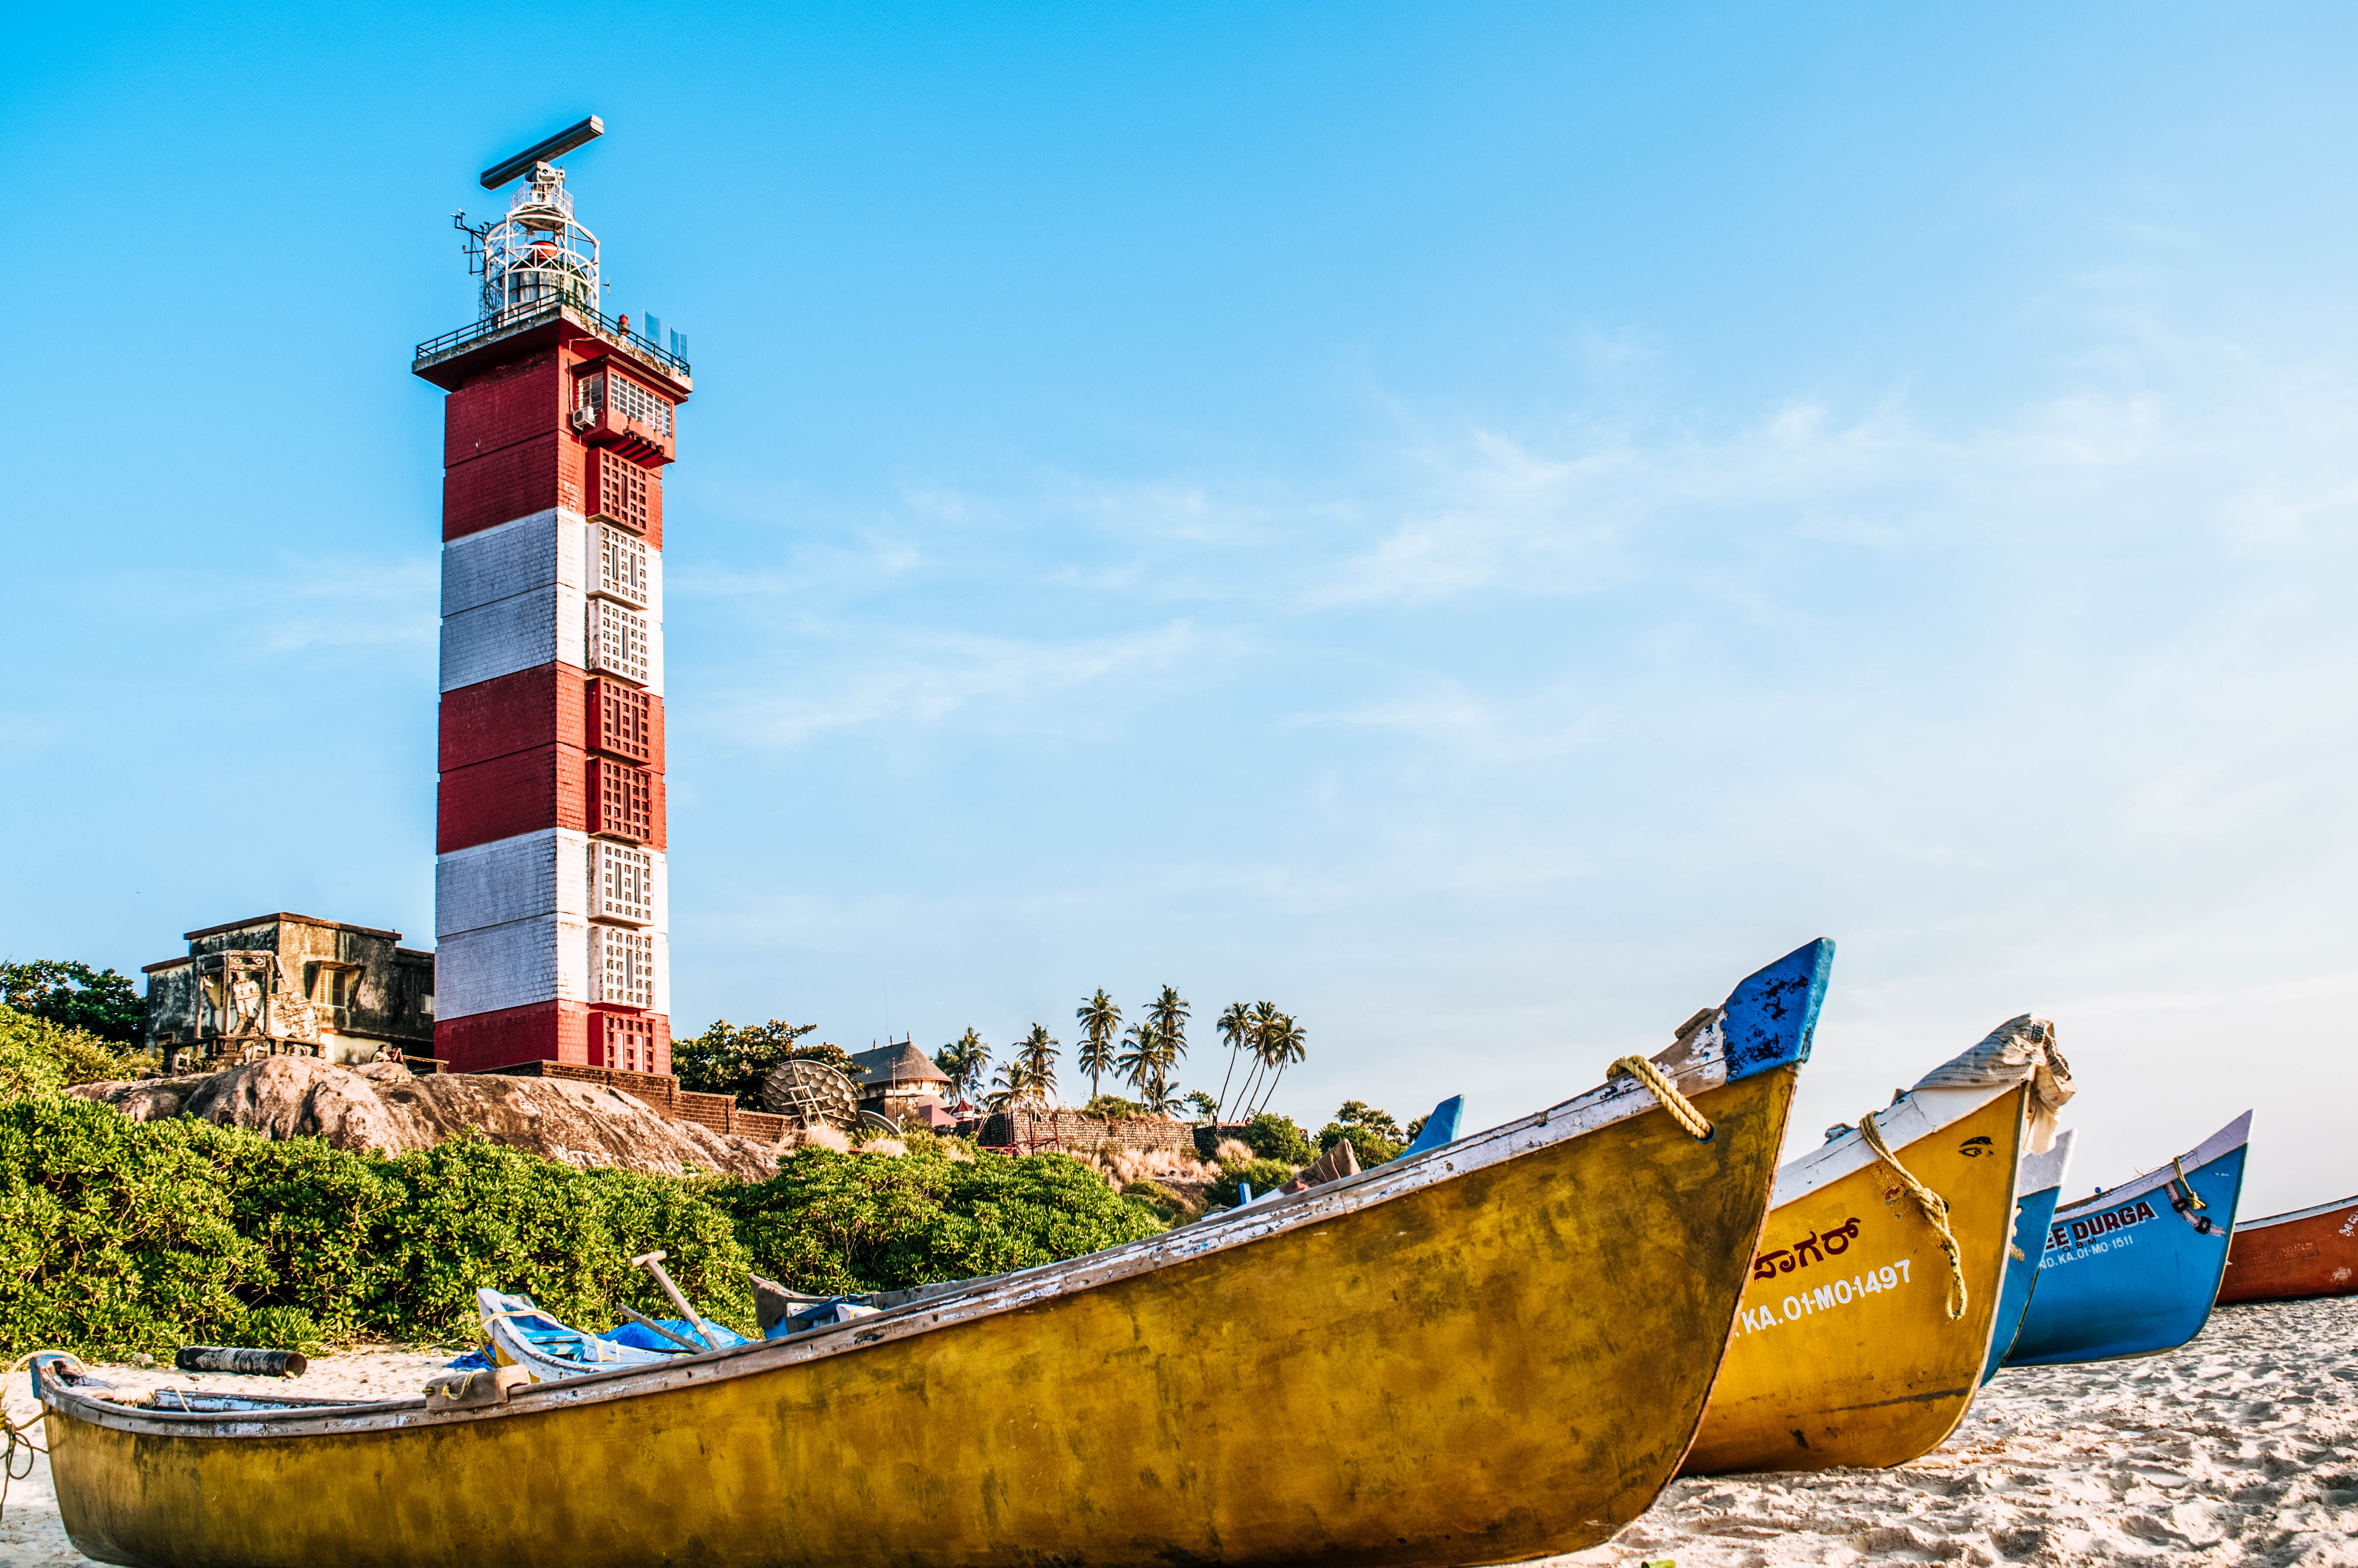
\includegraphics[width=\columnwidth]{./figures/image_lh.jpg}
    \caption{NITK has beach}
    \label{fig:lighthouse}
\end{figure}

\column{0.55\textwidth}
NITK has beach! Beach is cool!

\end{columns}
\end{frame}
%---------------------------------------------------------


\end{document}